\chapter{Controls}
\label{ch:controls}
Control systems are responsible for computing the commands necessary for actuators to cause the trajectory of a system to go from its current state to a desired state, or for answering the question "How do I get there?". There are many different methods that can be used to determine the output commands. One of the more popular and widely implemented control systems is the PID (Proportional, Integral, Differential) controller. Model based controllers utilize knowledge of the physics of the system to compute appropriate output commands. The robots in these experiments originally used PID controllers for position and heading control and were later tested with a model based contoller that takes advantage of Lyapunov stability theory.

\section{PID}
\label{sec:pid}
PID controllers use the current state estimate to determine the errors between the desired state and the current state. The goal of the PID controller is to drive those errors to zero based on a number of criteria including rise time, settling time, steady state error and overshoot as shown in Figure \ref{fig:pid} where the green line is the ideal output while the blue and purple lines are typical results. The orange line shows what happens when a system becomes unstable. Point $m$ represents the desired state, $m-n$ represents steady state error, point $a$ is the rise time for the blue line and point $b$ is the settling time for the blue line.

\begin{figure}[ht!]
	\centering
	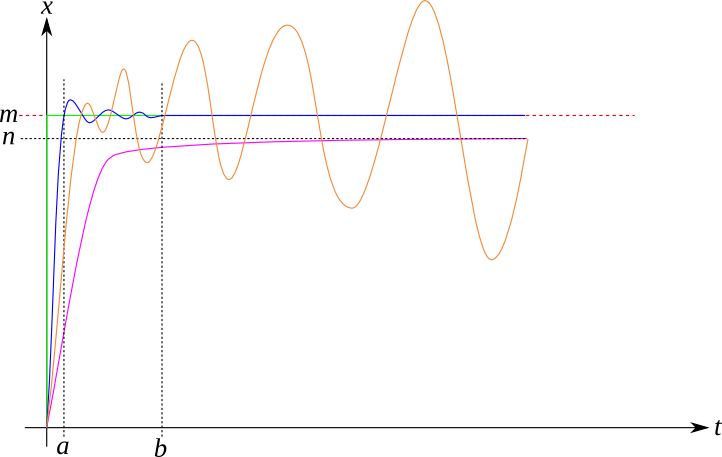
\includegraphics[width=.85\textwidth]{images/pid}
	\caption{PID Controller Responses} 
	\label{fig:pid}
\end{figure}

There are separate PID controllers used for robot distance ($e$) and heading errors ($\psi$). The process used to compute an output command using a PID controller uses three separate errors and a gain for each of the distance and heading errors. Looking at the PID controller for heading the errors are
\begin{align*}
%\label{eq:piderrors}
\begin{split}
E_P &= \psi_{\text{ref}_k} - \psi_k \\
E_I &= \sum_{i=0}^{k}E_{P_i}*\Delta_T \\
E_D &= \frac{\psi_k - \psi_{k-1}}{\Delta_T}
\end{split}
\end{align*}
where $\psi_{\text{ref}_k}$ is the desired heading at the current time, $\psi_k$ is the current heading estimate, $\psi_{k-1}$ is the previous heading estimate and $\Delta_T$ is the time elapsed since the last PID control calculation was performed. The contribution of each error is then weighted by a gain to obtain the final output command, $u$, such that
\begin{align*}
%\label{eq:pidcommand}
u = K_P*E_P + K_I*E_I + K_D*E_D
\end{align*}
where $K_P$ is the proportional gain, $K_I$ is the integral gain and $K_D$ is the differential gain.

The only parameters available to tune PID controllers for performance are the gains. There are some rules of thumb for tuning gains properly as described in \cite{ZeiglerNichols42} that can work as a good starting point, along with a basic knowledge of what the effects are of modifying the different gains as summarized in Table \ref{tab:PIDGainEffects}. The difficulty in using PID controllers for the small robots used in these experiments is that the gains must be tuned for specific operating scenarios so that a set of gains that work well at full speed on asphalt do not work at all when the robot is driving in soft sand at any velocity. PID controllers work best when they only have to reject a small range of disturbances, however the small robots are required to be operated in environments with a large range of disturbances.

When the characteristics of a robot are changed the PID gains must also be modified to reflect those changes. These characteristics include mass, center of mass, particular treads or motors and payloads, as these all affect the dynamics of the system. Gain scheduling is the process of tuning a system to use a different set of gains based on the operating environment or characteristics of the robot and is very time consuming. This motivates the search for a better control system for these small robots.

Table \ref{tab:PIDGainEffects} shows how increasing the different gain values affects the performance of the controller output in terms of rise time, overshoot, settling time and steady state error. It can be seen that a large amount of coupling exists between the gains and attempting to fix one aspect of the controller output can have unintended consequences that cause other aspects of controller output to perform suboptimally. This is in contrast to the gains that arise for model based controllers as seen in Chapter \ref{sec:lyapunovTrajectoryConvergence}.

\begin{table}[ht!]
\caption{Effects on Controller Output of Modifying PID Gains}
\small
\centering
\begin{tabular}{@{}llllr@{}} \toprule
Parameter    & Rise Time      & Overshoot & Settling Time & Steady State Error \\ \midrule
$K_p$        & Decrease       & Increase  & Small Change  & Decrease \\
$K_i$        & Decrease       & Increase  & Increase      & Eliminate \\
$K_d$        & Small Decrease & Decrease  & Decrease      & None \\ \bottomrule
\end{tabular}
\label{tab:PIDGainEffects}
\end{table}

\section{Model Based Controller}
\label{sec:lyapunov}
An alternative control method to using classical PID controllers is to use model based controllers based on Lyapunov stability theory. An intuitive way to conceptualize controllers based on this stabilty theory is by thinking of them as decreasing the overall energy of a system, even when the variables involved in the control Lyapunov functions do not represent energy \cite{Khalil02}.

The theorem for Lyapunov stability states that for an equilibrium point $x=0$ and a domain $D\subset\mathbb{R}^n$ that contains $x=0$ and for which there is a function $V:D\to\mathbb{R}$ that is continuously differentiable and has the following properties 
\begin{align*}
%\label{eq:lyapunovTheorem}
\begin{split}
V(0) &= 0 \\
V(x) &> 0 \in D-\{0\} \\
\dot{V}(x) &\leq 0 \in D-\{0\}
\end{split}
\end{align*}
then the equilibrium point $x=0$ is stable. Additionally, if
\begin{align*}
%\label{eq:lyapunovAsymptoticStability}
\dot{V}(x) < 0 \in D - \{0\}
\end{align*}
then $x=0$ is asymptotically stable.

It is not always possible to find such a control Lyapunov function $V$ but when one is found then this theorem holds and the "energy" of the system will always be positive and decreasing. The "energy" can consist of any variables that make $V(0) = 0$ and $V(x) > 0$ and often consist of a combination of the errors that are to be minimized in a system. In that case the errors are always decreasing since $\dot{V}(x) < 0$ and the system will reach the desired state.

\subsection{Unicycle-like Robot Kinematics}
\label{sec:unicycleKinematics}
Several groups have implemented model-based controllers rooted in Lyapunov stability theory in simulation including \cite{Aicardi_UnicycleLyapunov95, Gulati08, Rusu05RobotuxLyapunov, Aicardi94, MicaelliLyapunov93} but only recently have these results been applied to actual robots \cite{NuchterLyapunov07, KimLyapunov05, Lapierre06, Lapierre07}. All of these groups describe a method for constructing a control Lyapunov function based on the kinematics of a differential drive robot, similar in nature to the small robots considered in these experiments and typically referred to as a unicycle-like robots in the literature.

\begin{figure}[ht!]
	\centering
	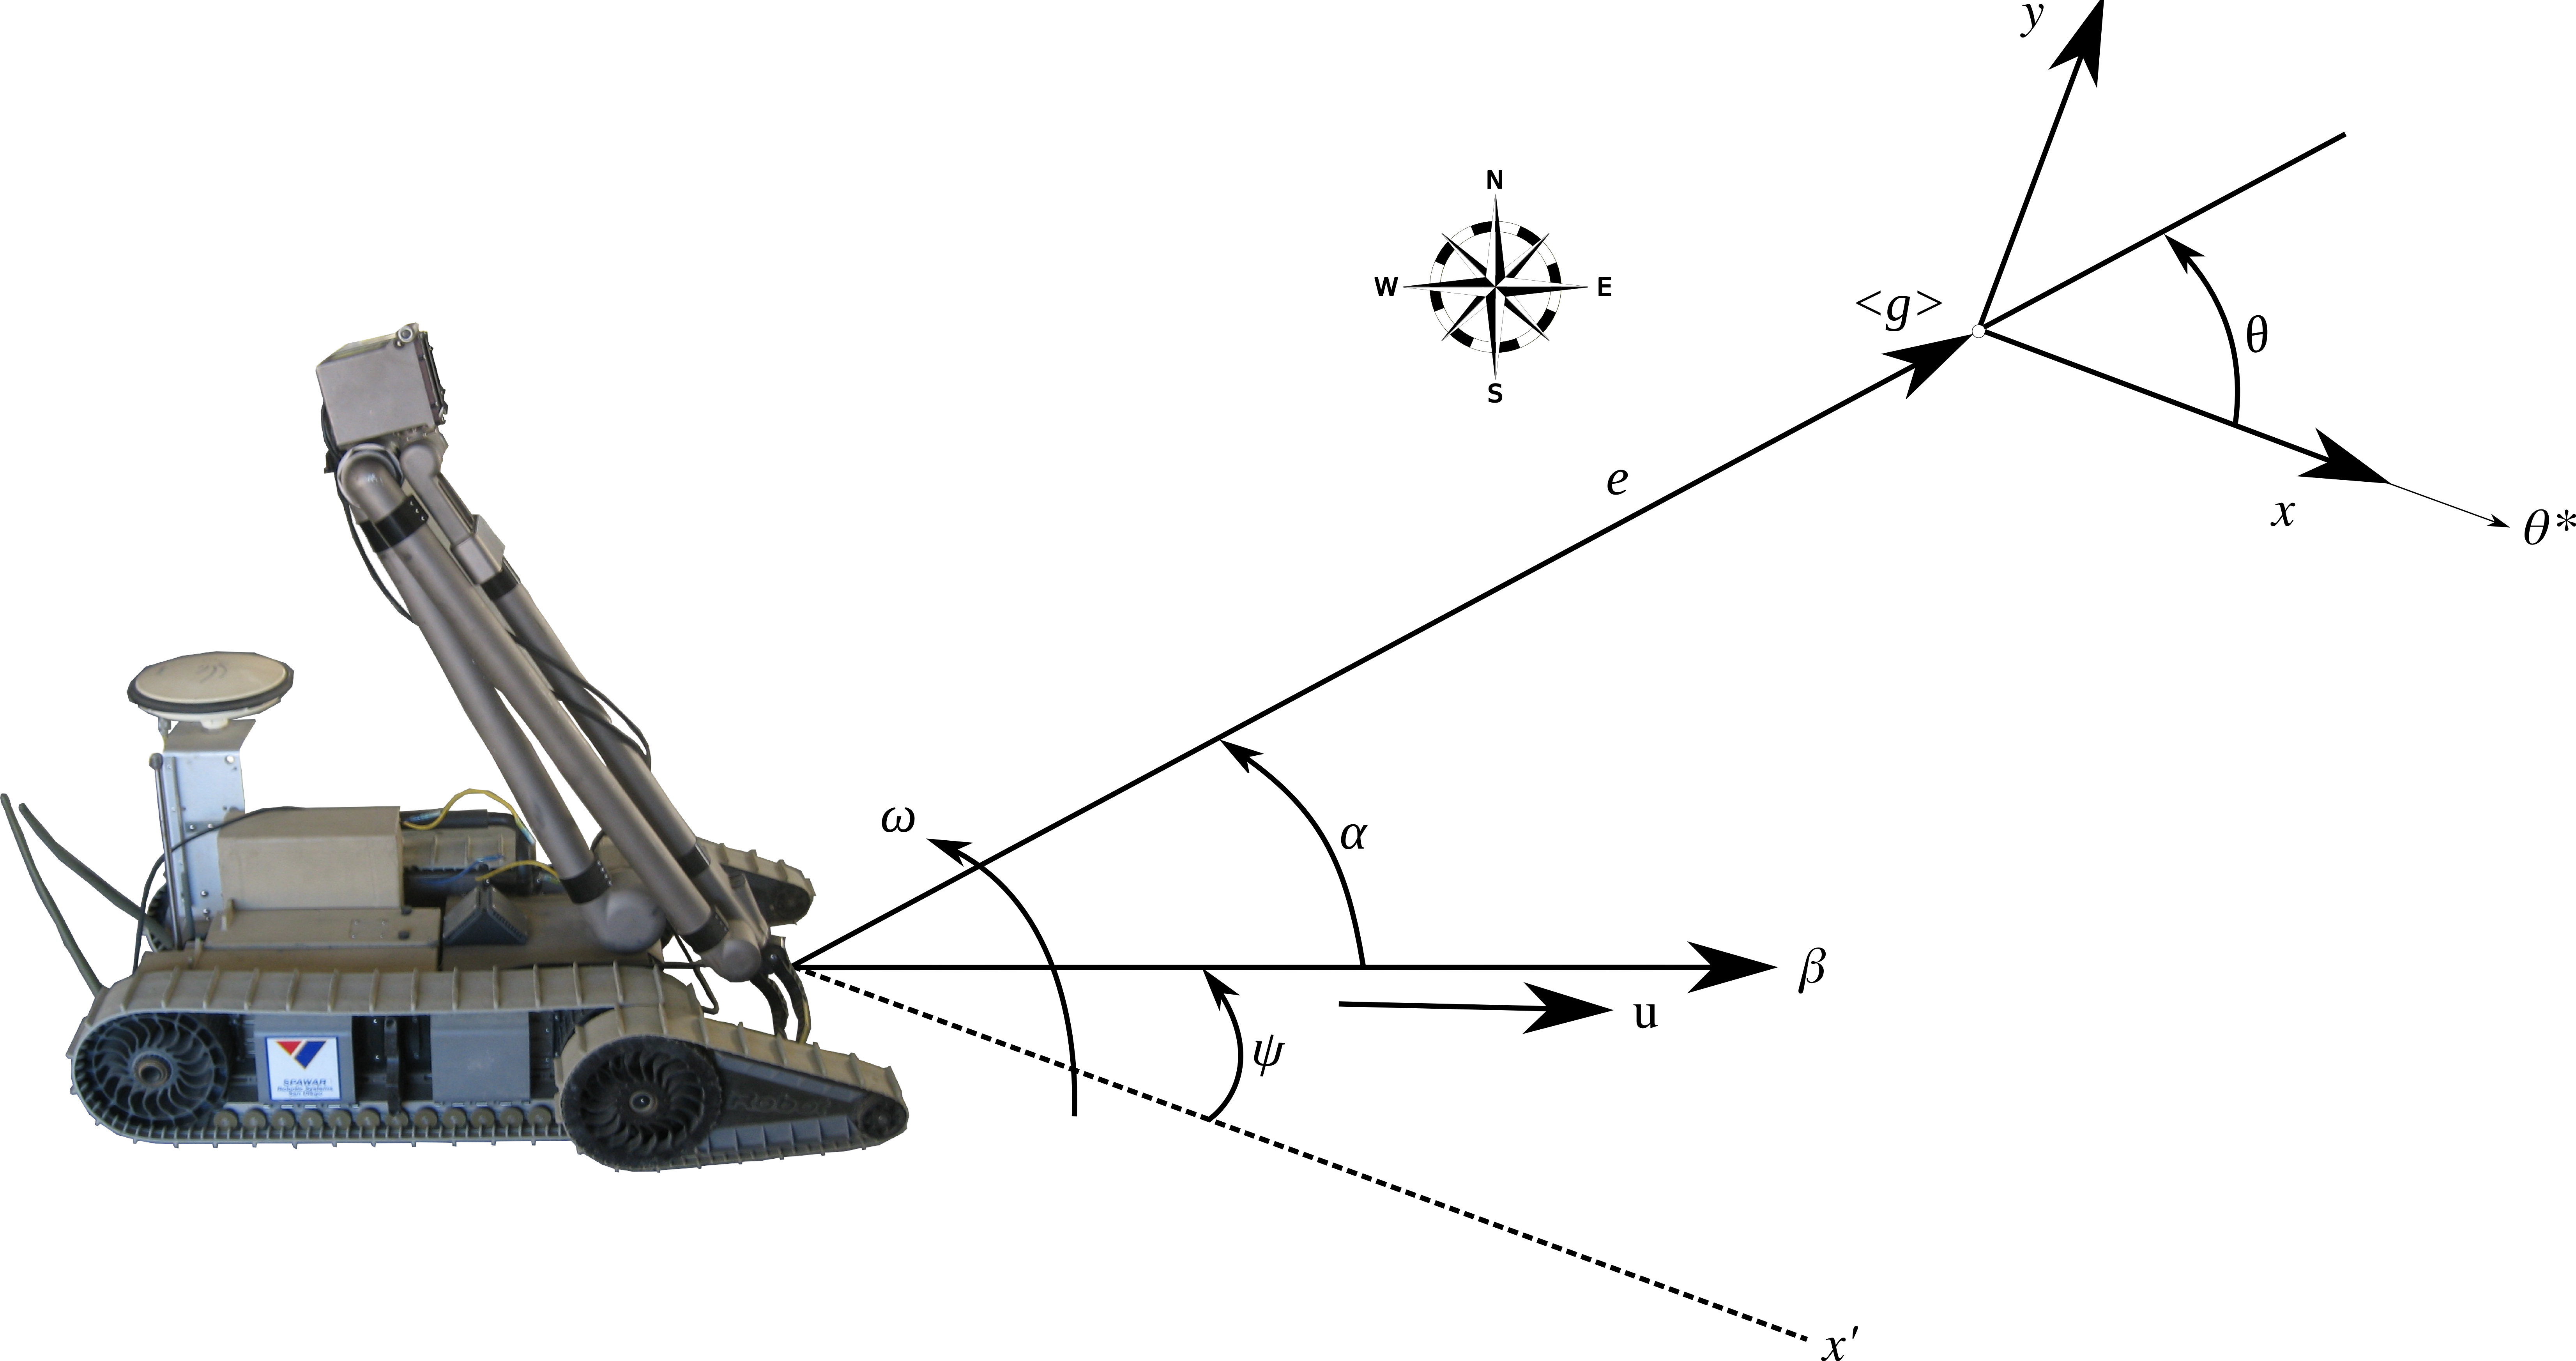
\includegraphics[width=.95\textwidth]{images/packbotlyapunov}
	\caption{PackBot Coordinate System for Model Based Controller}
	\label{fig:pblyapunov}
\end{figure}

Figure \ref{fig:pblyapunov} will be used as the basis for the equations that follow and will be explained in further detail here. Given a robot at some arbitrary initial position we want it to move to a goal position with a specific heading where the goal position is the origin of the $<g>$ coordinate system and the desired heading is along the $x$-axis of the $<g>$ coordinate system labeled $\theta^\star$. The states that define the robot's current position, heading, and linear and angular velocities are calculated using the Kalman filter of Chapter \ref{sec:extendedkf} whereas the goal position and heading are given as inputs to the robot. Note that the linear velocity is given by $u$ and the angular velocity by $\omega$. The control system attempts to force three separate errors to zero:
\begin{itemize}
\item $e$, the magnitude of the translation error vector as measured between the current position and goal position,
\item $\theta$, the angle between the desired heading and the translational error vector $e$,
\item $\alpha$, the angle between the current heading and the translational error vector $e$.
\end{itemize}

Additional variables used to calculate the errors include
\begin{itemize}
\item $\theta^\star$, the target heading in the global coordinate system which is aligned with the $x$-axis,
\item $\beta$, the current heading of the robot in the global coordinate system,
\item $\phi$, the difference between the target heading and the current heading in the global coordinate system.
\end{itemize}

Since unicycle-like robots exhibit non-holonomic constraints (they are only able to move forwards or backwards along the direction of their current heading and are not able to perform strafing maneuvers) it is necessary to use all three errors in the control system. The errors can all be calculated using the inputs to the robot of a goal position and goal heading and the state estimate output of the Kalman filter.

A kinematic model of the robot is used to predict how the robot moves without considering the effects of the mass of the robot or outside forces (such as friction between the robot tracks and the ground) acting on the robot with
\begin{align}
\label{eq:lyapunovkinematics1}
\begin{split}
\dot{x} &= u\cos(\phi) \\
\dot{y} &= u\sin(\phi) \\
\dot{\phi} &= \omega.
\end{split}
\end{align}
The expressions in (\ref{eq:lyapunovkinematics1}) are then converted to a polar coordinate representation via a coordinate transformation and give expressions for the errors that the control system is attempting to drive to zero such that
\begin{align}
\label{eq:lyapunovPolar}
\begin{split}
e &= \sqrt{x^2+y^2} \\
\theta &= \atanh(y,x) \\
\alpha &= \theta - \phi.
\end{split}
\end{align}
Combining (\ref{eq:lyapunovPolar}) with (\ref{eq:lyapunovkinematics1}) results in
\begin{align*}
%\label{eq:lyapunovkinematics3}
\begin{split}
\dot{e} &= -u*\cos(\theta-\phi) \\
\dot{\theta} &= u\frac{\sin\alpha}{e} \\
\dot{\phi} &= \omega.
\end{split}
\end{align*}
Finally, replacing $\alpha$ with $\theta-\phi$ results in a kinematic model of
\begin{align}
\label{eq:lyapunovkinematics}
\begin{split}
\dot{e} &= -u\cos\alpha \\
\dot{\alpha} &= -\omega + u\frac{\sin\alpha}{e} \\
\dot{\theta} &= u\frac{\sin\alpha}{e}.
\end{split}
\end{align}

\subsection{Control Lyapunov Function}
\label{sec:controllyapunov}
The control Lyapunov function is selected to be positive, contain all three error states and separate the distance error from the angle errors and is given by
\begin{align*}
%\label{eq:lyapunovfunction}
V = V_1 + V_2 = \frac{1}{2}\lambda e^2 + \frac{1}{2}\left(\alpha^2+h\theta^2\right)
\end{align*}
where $\lambda$ and $h$ are positive constants that can be used to tune the controller output (see Chapter \ref{sec:lyapunovTrajectoryConvergence}). Using the kinematics equations in (\ref{eq:lyapunovkinematics}) the derivative of each term of the candidate control Lyapunov function can be found as
\begin{align}
\label{eq:Vderivatives}
\begin{split}
\dot{V}_1 &= \lambda e\dot{e} = \lambda e (-u\cos\alpha) = -\lambda eu\cos\alpha \\
\dot{V}_2 &= \alpha\dot{\alpha}+h\theta\dot{\theta} \\
&= -\alpha\omega + \alpha u\frac{\sin\alpha}{e} + h\theta u\frac{\sin\alpha}{e} \\
&= \alpha\left(-\omega + u\frac{\sin\alpha}{e} + h\theta u\frac{1}{\alpha}\frac{\sin\alpha}{e}\right) \\
&= \alpha\left(-\omega + u\frac{\sin\alpha}{\alpha}\frac{(\alpha+h\theta)}{e}\right)
\end{split}
\end{align}
and from (\ref{eq:Vderivatives}) the total derivative is found as
\begin{align}
\label{eq:lyapunovfunctionderivative}
\begin{split}
\dot{V} &= \dot{V}_1 + \dot{V}_2 = -\lambda e u\cos\alpha + \alpha\left(-\omega+u\frac{\sin\alpha}{\alpha}\frac{(\alpha+h\theta)}{e}\right).
\end{split}
\end{align}

Now it needs to be shown that $\dot{V}\leq0$ which can be done by showing that $\dot{V}_1\leq0$ and $\dot{V}_2\leq0$. This is true for $\dot{V}_1$ if $u$ takes the form
\begin{align}
\label{eq:lyapunovu}
u = \gamma e\cos\alpha
\end{align}
where $\gamma$ is a positive constant different from $\lambda$. Substituting this value of $u$ into (\ref{eq:Vderivatives}) results in
\begin{align}
\label{eq:V1dotfinal}
\dot{V}_1 = -\lambda eu\cos\alpha = -\lambda\gamma e^2\cos^2\alpha \leq 0.
\end{align}
Since $V_1\geq0$ and $\dot{V}_1\leq0$ we have that $V_1$ converges asymptotically to a positive defined limit.

Replacing $u$ in the expression for $\dot{V}_2$ in (\ref{eq:Vderivatives}) results in
\begin{align}
\label{eq:V2dotreplaceu}
\begin{split}
\dot{V}_2 &= \alpha\left(-\omega+u\frac{\sin\alpha}{\alpha}\frac{(\alpha+h\theta)}{e}\right) \\
&= \alpha\left(-\omega+\gamma e\frac{\cos\alpha\sin\alpha}{\alpha}\frac{(\alpha+h\theta)}{e}\right) \\
&= \alpha\left(-\omega+\gamma(\alpha+h\theta)\frac{\cos\alpha\sin\alpha}{\alpha}\right).
\end{split}
\end{align}

Similarly, $\dot{V}_2$ is negative semidefinite if $\omega$ takes the form
\begin{align}
\label{eq:lyapunovomega}
\begin{split}
\omega &= k\alpha + \gamma\frac{\cos\alpha\sin\alpha}{\alpha}\left(\alpha+h\theta\right)
\end{split}
\end{align}
where $k$ is a positive constant. Substituting this value of $\omega$ into (\ref{eq:V2dotreplaceu}) gives
\begin{align}
\label{eq:V2dotfinal}
\begin{split}
\dot{V}_2 &= \alpha\left(-k\alpha-\gamma\frac{\cos\alpha\sin\alpha}{\alpha}(\alpha+h\theta) + \gamma\frac{\cos\alpha\sin\alpha}{\alpha}(\alpha+h\theta)\right) \\
&= -k\alpha^2 \leq 0
\end{split}
\end{align}
and $V_2$ converges asymptotically to a positive defined limit.

Substituting $\dot{V}_1$ from (\ref{eq:V1dotfinal}) and $\dot{V}_2$ from (\ref{eq:V2dotfinal}) into the expression for $\dot{V}$ (\ref{eq:lyapunovfunctionderivative}) yields
\begin{align*}
%\label{eq:Vfinal}
\dot{V} = \dot{V}_1 + \dot{V}_2 = -\lambda\gamma e^2\cos^2\alpha - k\alpha^2 \leq 0.
\end{align*}
This expression is equal to zero if and only if $\alpha=0$ \textit{and} $e=0$, which only occurs when the robot has reached its goal pose. Therefore, at any point along the robots trajectory other than the goal point this function is negative definite and is asymptotically stable.

Using the expressions for $u$ in (\ref{eq:lyapunovu}) and $\omega$ in (\ref{eq:lyapunovomega}) and substituting those values back into the kinematic model from (\ref{eq:lyapunovkinematics}) gives
\begin{align}
\label{eq:lyapunovfinalkinematics}
\begin{split}
\dot{e} &= -u\cos\alpha = -\gamma e\cos^2\alpha \\
\dot{\alpha} &= -\omega + u\frac{\sin\alpha}{e} \\
&= -(k\alpha+\gamma\frac{\cos\alpha\sin\alpha}{\alpha}(\alpha+h\theta))+\gamma e\cos\alpha\frac{\sin\alpha}{e} \\
&= -k\alpha-\gamma\cos\alpha\sin\alpha+\gamma\cos\alpha\sin\alpha-\gamma h\theta\frac{\cos\alpha\sin\alpha}{\alpha} \\
&= -\left(k\alpha + \gamma h\theta\frac{\cos\alpha\sin\alpha}{\alpha}\right) \\
\dot{\theta} &= u\frac{\sin\alpha}{e} = \gamma e\cos\alpha\frac{\sin\alpha}{e} = \gamma\cos\alpha\sin\alpha
\end{split}
\end{align}

Combining (\ref{eq:lyapunovu}) and (\ref{eq:lyapunovomega}) gives the following control law to replace the PID controller from Chapter \ref{sec:pid}:
\begin{align}
\label{eq:lyapunovControlLaw}
\begin{split}
u &= \gamma e\cos\alpha \\
\omega &= k\alpha + \gamma\frac{\cos\alpha\sin\alpha}{\alpha}\left(\alpha+h\theta\right)
\end{split}
\end{align}

\subsection{Calculating Control Law Variables}
\label{sec:lyapunovVariables}
The method used to calculate the variables needed for the control law in (\ref{eq:lyapunovControlLaw}) based on Figure \ref{fig:pblyapunov} is:
\begin{enumerate}
\item $dx$ is the vertical component of the error vector $e$ since the $x-$axis is forward of the vehicle as seen in Figure \ref{fig:pblyapunov}.
\item $dy$ is the horizontal component of the error vector $e$ as seen in Figure \ref{fig:pblyapunov}.
\item $e$ can be calculated in several different ways:
\begin{itemize}
\item Use a path planner to set a carrot out in front of the robot on the path between the current position of the robot and the goal point. That carrot moves along to the next path segment when the robot gets close enough to the end waypoint of the current path segment if the current waypoint is not the final waypoint. This could cause $e$ to be much smaller than it actually is so $\alpha$ will be corrected sooner than it should be and an additional problem could occur if the robot tries to correct $\theta$ too early.
\item Use $\sqrt{dx^2 + dy^2}$ to get the distance to the end waypoint on the current path segment. This will cause the robot to slow down as it reaches every waypoint, even intermediate ones. Conversely, if $e$ is very large then $u$ could grow to be too large as well and necessitate the use of a limiting value for $u$.
\item Combine the two methods and use the actual distance to the end waypoint of the current path segment until that value is less than the distance to the carrot and then use the carrot distance for $e$.
\end{itemize}
\item $\psi$ is the current heading of the robot in the world coordinate frame and is calculated in the Kalman filter code based on the results from Chapter \ref{ch:estimation}.
\item $\alpha$ is the angle between the current heading of the robot $\psi$ and the error vector $e$ where the angle of the error vector $e$ is from the current position to the waypoint and found as $\tan^{-1}\left(\frac{dy}{dx}\right)$. The desired angle error is $\alpha = \tan^{-1}\left(\frac{dy}{dx}\right) - \psi$.
\item $\theta^\star$ is the desired heading in the global coordinate system and there are multiple ways that it \textit{could} be set.
\begin{itemize}
\item $\theta^\star=0$ sets the desired heading as North and $\theta^\star=\pi$ sets it as South.
\item $\theta^\star=\psi$ would make the desired heading be the same as whatever the current heading happens to be.
\item $\theta^\star$ can be sent in as an additional parameter of a waypoint, say from MOCU via JAUS.
\item Look at the current waypoint and next waypoint positions. If there is no next waypoint then just go straight to the current waypoint with $\theta^\star=\psi$. If there is a next waypoint then $\theta^\star$ could be the angle from the current waypoint to the next waypoint or splitting the difference between heading to the current and next waypoints.
\end{itemize}
\item $\phi=\theta^\star-\psi$.
\item $\theta=\alpha + \phi$.
\end{enumerate}
Note that all of the angle variables need to be normalized so that they are in the range $(-\pi,\pi]$.

\subsection{Effect of Gains on Trajectory}
\label{sec:lyapunovTrajectoryConvergence}
The gains $h$, $k$ and $\gamma$ in the control law (\ref{eq:lyapunovControlLaw}) determine the resulting trajectory that the robot will use when driving from its current position to the goal point and heading. The first thing to notice is that the linear velocity is at a maximum when the angle error $\alpha=0$ since that leads to $\cos(\alpha)=1$ and $u_{\text{max}}=e\gamma$. As discussed in Chapter \ref{sec:lyapunovVariables} a carrot can be set by the path planner to limit the maximum error distance $e$ so that $e$ is bounded. When that is the case the maximum linear velocity is proportional to the gain $\gamma$. For example, if the carrot has a maximum lookahead distance of $10m$ and $\gamma=0.2$ then $u_{\text{max}}=10*0.2=2\tfrac{m}{s}$ which is a reasonable limit for a PackBot.

There are many ways to select what values the gains $h$ and $k$ should take, especially once $\gamma$ is set, and some of the properties of the kinematics equations (\ref{eq:lyapunovfinalkinematics}) as the angle errors $(\alpha, \theta)$ approach $(0, 0)$ are helpful in making those selections as the system involving the errors to be minimized is approximately linear. The key to this linearization is to notice that when $\alpha$ is near zero several terms in (\ref{eq:lyapunovfinalkinematics}) cancel out since $\alpha\to0\Rightarrow \alpha=\cos(\alpha)*\sin(\alpha)=\sin(\alpha)$ as seen in Figure \ref{fig:plotSinCos}. When that is the case the following linear approximation holds:
\begin{align}
\label{eq:lyapunovLinearSystem}
\begin{split}
\left[\begin{array}{c} \dot{\alpha} \\ \dot{\theta} \end{array}\right]
&= \underbrace{\left[\begin{array}{c c} -k & -h\gamma \\ \gamma & 0 \end{array}\right]}_{A}
\left[\begin{array}{c} \alpha \\ \theta \end{array}\right] \\
\dot{e} &= -\gamma e
\end{split}
\end{align}
with linear output equations
\begin{align}
\label{eq:lyapunovLinearOutput}
\begin{split}
u &= \gamma e \\
\omega &= (k+\gamma)\alpha + h\gamma\theta.
\end{split}
\end{align}

\begin{figure}[ht!]
	\centering
	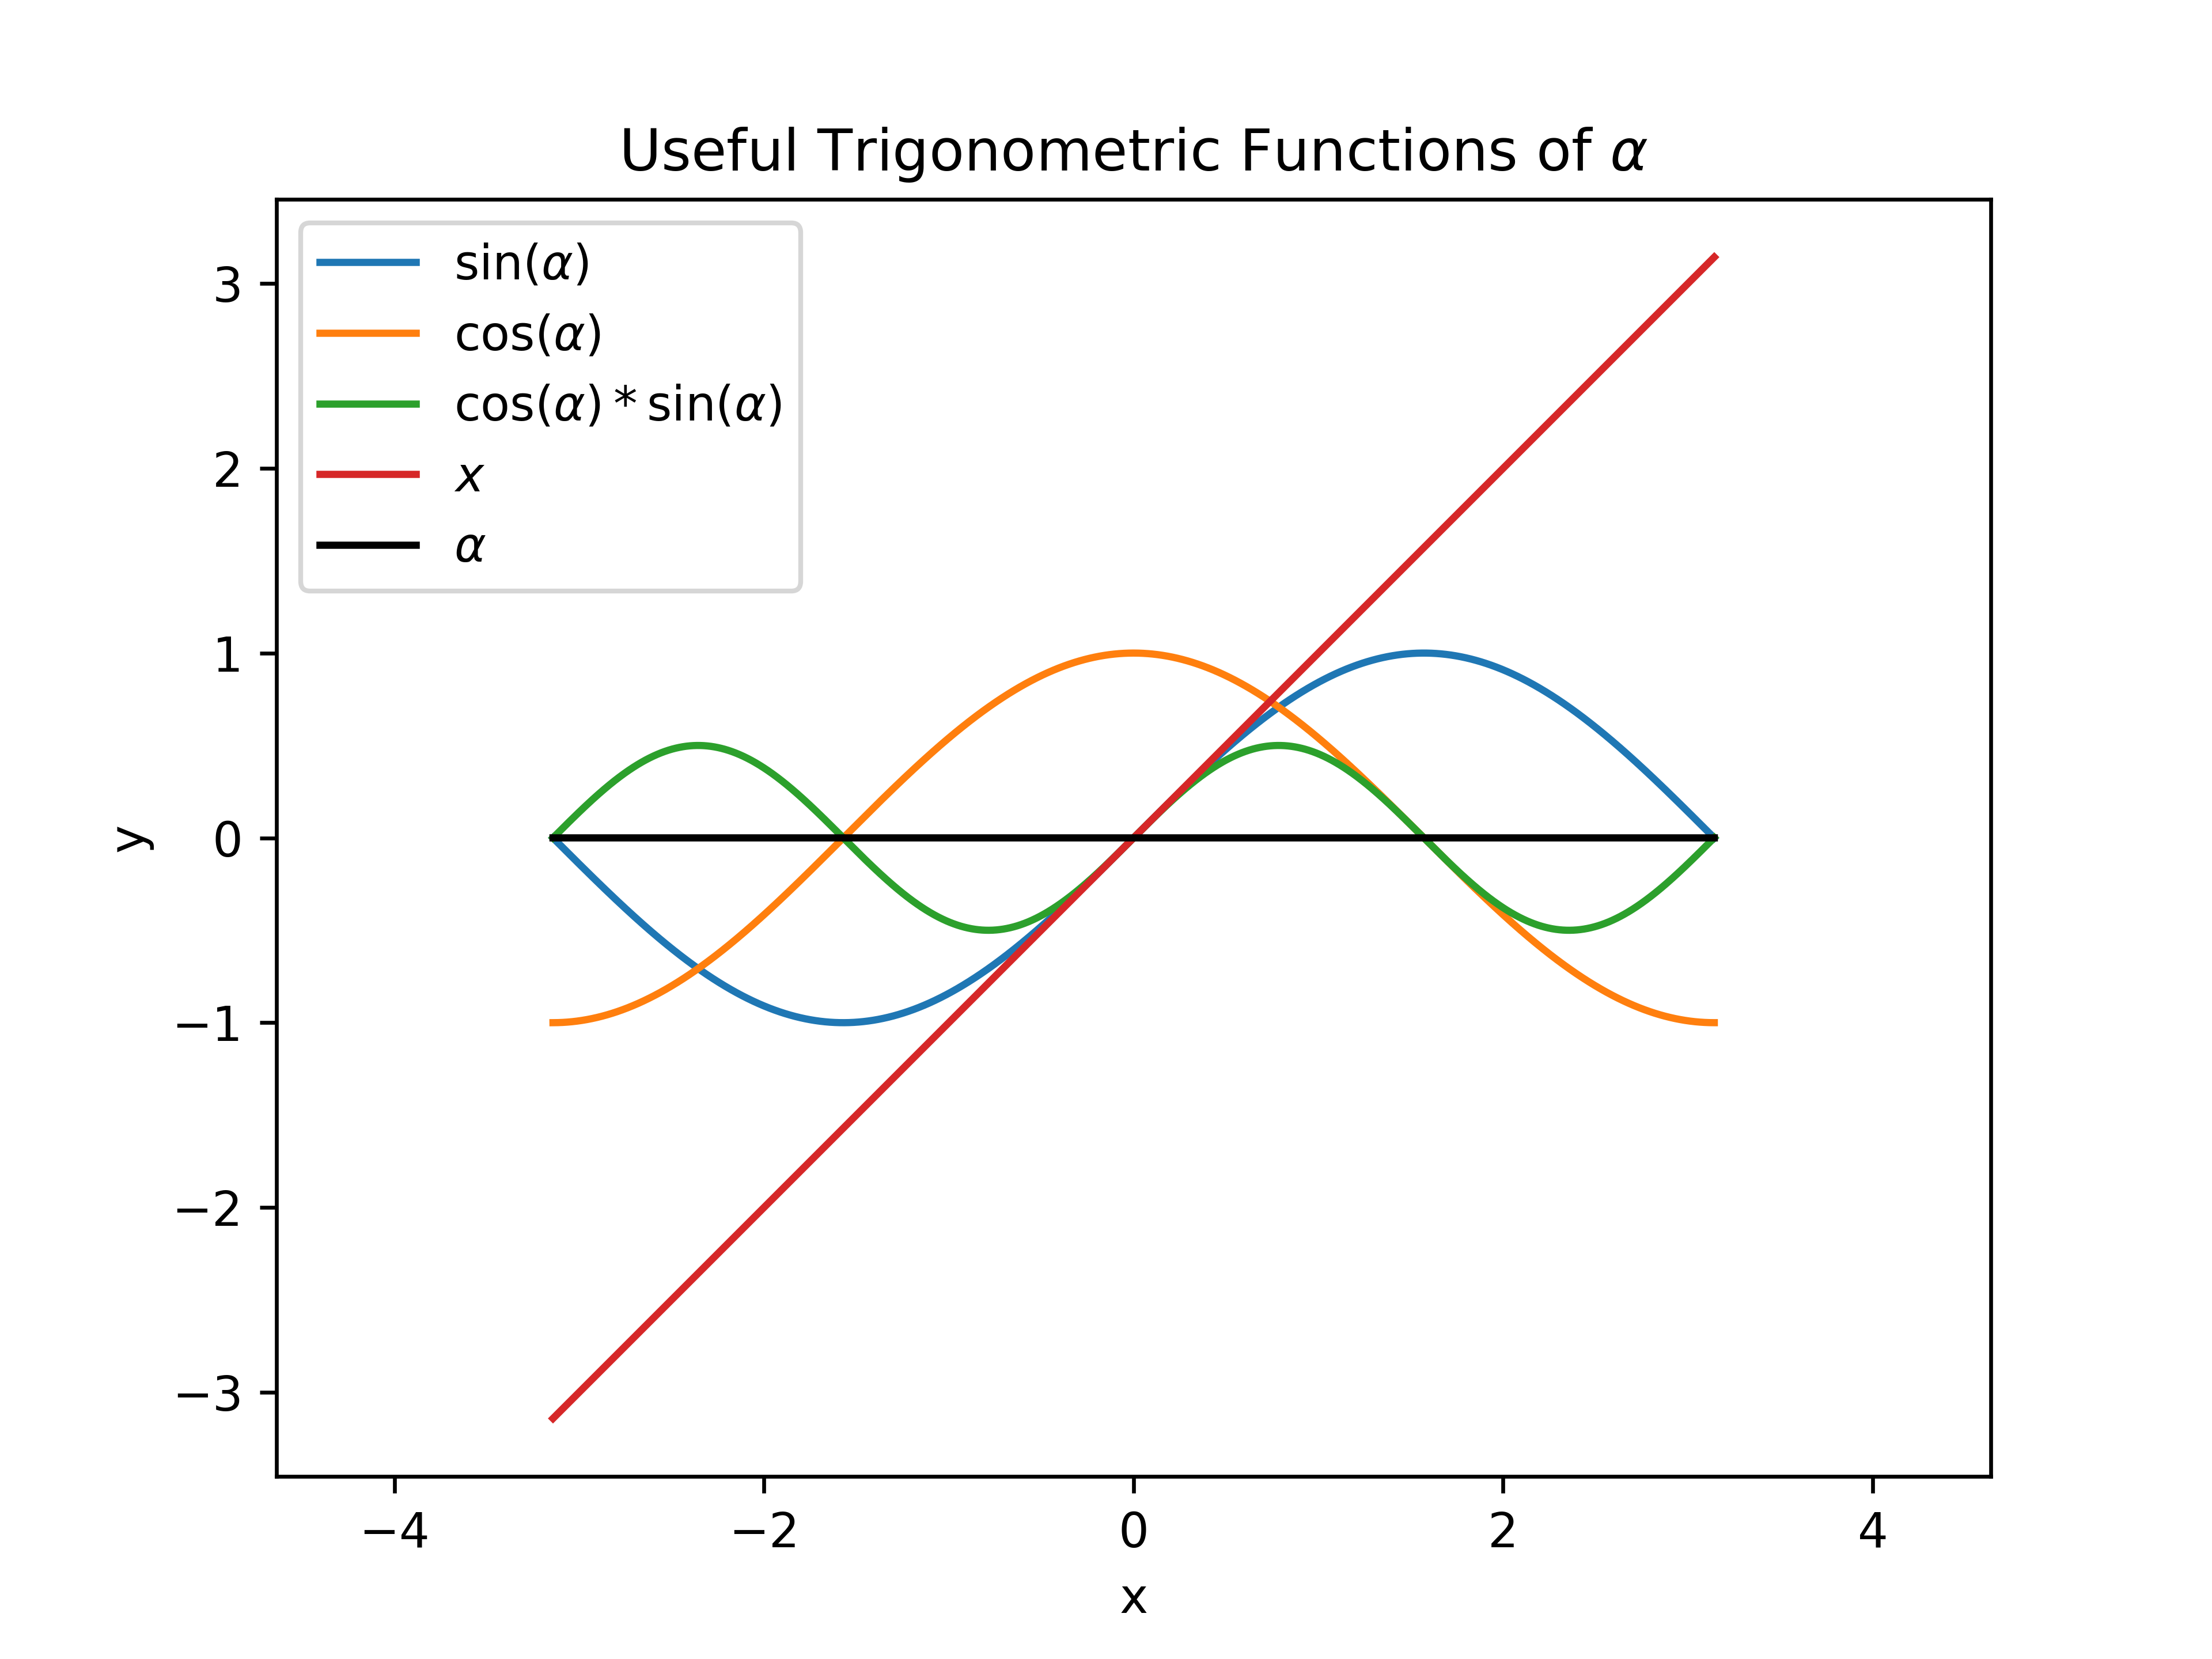
\includegraphics[width=.75\textwidth]{images/plotSinCos}
	\caption{Plot of $\alpha$, $\sin\alpha$, $\cos\alpha$ and $\sin\alpha*\cos\alpha$}
	\label{fig:plotSinCos}
\end{figure}

This shows that, in the neighborhood of $(\alpha, \theta)=(0, 0)$, the distance error $e$ converges at a rate of $\text{exp}(-\gamma t)$ while the angle errors converge at a rate of $\text{exp}(-\sigma t)$ where $-\sigma$ is the real part of the dominant pole of the linear system $A$ in (\ref{eq:lyapunovLinearSystem}) which can be found from the eigenvalues of $A$. The reason that the errors converge at those rates is that, for the distance error, $e=\text{exp}(-\gamma t)$ is a solution to the equation $\dot{e}=-\gamma e$ since 
\begin{align*}
\tfrac{d}{dt}e=\tfrac{d}{dt}\text{exp}(-\gamma t) = -\gamma \text{exp}(-\gamma t)=-\gamma e.
\end{align*}
Similarly, the behavior of the angle errors is related to the matrix $A$ and nonsingular matrices can be factored into the form $A=S\Lambda S^{-1}$ where $S$ contains the eigenvectors of $A$ and $\Lambda$ is a diagonal matrix containing the eigenvalues of $A$. The solution to the differential equation is
\begin{align*}
\left[\begin{array}{c} \dot{\alpha} \\ \dot{\theta} \end{array}\right] = \text{exp}(At)=\text{exp}(S\Lambda S^{-1}t)=S\text{exp}(\Lambda t)S^{-1}
\end{align*}
and $\dot{\alpha}$ has the solution $\alpha=\text{exp}(-\lambda_1 t)$ and $\dot{\theta}$ has the solution $\theta=\text{exp}(-\lambda_2 t)$.

Three reasonable design considerations in selecting the gains are:
\begin{itemize}
\item limit the maximum linear velocity,
\item find critically damped gains,
\item have angle errors converge before distance error.
\end{itemize}
Limiting the maximum linear velocity has been discussed already and involves the selection of $\gamma$. The damping of the system $A$ is determined by
\begin{align*}
\zeta = \frac{\lambda_1(A)}{\lambda_2(A)}
\end{align*}
and the gains are critically damped when $\zeta = 1 \Rightarrow \lambda_1(A)=\lambda_2(A)=\lambda$ so that both angle errors $\alpha$ and $\theta$ are converging to zero at the same rate. When the system is critically damped the angle errors will converge before the distance error if $\sigma>\gamma$ since that means the rate of convergence for the angle errors is greater than the rate of convergence for the distance error. In the case where the $A$ matrix is overdamped $\zeta > 1 \Rightarrow \lambda_1(A) > \lambda_2(A)$ then $\alpha$ will converge to zero before $\theta$ and conversely when $A$ is underdamped $\zeta < 1$ and $\theta$ converges before $\alpha$.

By selecting the gains to satisfy the design considerations above the robot will align itself with the goal heading before arriving at the goal point and will smoothly decrease its linear velocity as it approaches the goal point. One alternative occurs when the distance error converges before the angle errors, $\gamma>\sigma$, and the robot will get to the goal point and then finish aligning with the goal heading which has several problems: (i) the robot does not look as intelligent since the trajectory does not appear to be as "natural" as the way a human would drive and (ii) rotating in place is typically a much more difficult maneuver for tracked robots to perform and increases the fatigue on the treads compared to turning while driving forward. The other alternative is that one angle error will converge before the other and this can lead to oscillations in heading since the two angle errors are coupled.

To deterministically discover gains that will satisfy the properties discussed two conditions must be met:
\begin{itemize}
\item $\zeta = 1$
\item $\sigma > \gamma$
\end{itemize}
For $\zeta=1$ it is necessary to first determine the eigenvalues of $A$.
\begin{align*}
&(A-\lambda I) = \left[\begin{array}{c c} -k-\lambda & -h\gamma \\ \gamma & -\lambda\end{array}\right] = 0 \\
\Rightarrow &(-k-\lambda)(-\lambda)+h\gamma^2 = 0 \\
\Rightarrow &\lambda^2 + k\lambda + h\gamma^2 = 0 \\
\Rightarrow &\lambda = \frac{-k\pm\sqrt{k^2-4h\gamma^2}}{2}
\end{align*}
For $\lambda_1(A)=\lambda_2(A)$ the term inside the square root must be equal to zero resulting in
\begin{align*}
&k^2 - 4h\gamma^2 = 0 \\
\Rightarrow &k = \sqrt{4h\gamma^2} = 2\gamma\sqrt{h}
\end{align*}
To find $\sigma>\gamma$ constrained by $k=2\gamma\sqrt{h}$ it is necessary to have
\begin{align*}
\sigma &= -\lambda = \tfrac{k}{2} > \gamma \\
\Rightarrow k &> 2\gamma
\end{align*}
The two equations can be combined to find $h$ such that
\begin{align*}
k &= 2\gamma\sqrt{h} > 2\gamma \\
\Rightarrow h &> 1
\end{align*}

Using this method any two gains can be selected and the third gain can be found which satisfies the above properties. For example, setting $\gamma=0.2$ to limit the maximum linear velocity and $h=1.1$ to keep it small but greater than one leads to $k=2\gamma\sqrt{h}=0.42$. From this it can be seen that $\lambda_1(A) = \lambda_2(A) = 0.21 \Rightarrow \zeta = 1$ so the system $A$ is critically damped and $\sigma = 0.21>0.2=\gamma$ so that the angle errors will converge before the distance error.

The model based controller developed in this Chapter along with the analysis of selecting appropriate gains replaces the original PID controller when answering the question "How do I get there?".
